\documentclass[12pt,a4paper]{ctexart}
\usepackage{geometry}
\geometry{left=2.5cm,right=2.5cm,top=2.0cm,bottom=2.5cm}
% \usepackage[english]{babel}
\usepackage{amsmath,amsthm}
\usepackage{amsfonts}
\usepackage[longend,ruled,linesnumbered]{algorithm2e}
\usepackage{fancyhdr}
\usepackage{array}
\usepackage{listings}
\usepackage{color}
\usepackage{graphicx}
\usepackage{minted}
\usepackage{float}
\usepackage[defaultmono]{droidsansmono}

\graphicspath{{pics/}}
\ctexset{today=small}
\definecolor{codebg}{rgb}{0.95,0.95,0.95}

\input{personal_info/info.tex}

\begin{document}
    \begin{titlepage}
        \heiti
        \vspace*{64pt}
        \begin{center}
            \fontsize{48pt}{0} 算法设计与分析\\
            \vspace*{36pt}
            \fontsize{48pt}{0}{实\quad 验\quad 报\quad 告}\\
            \vspace*{48pt}
            \LARGE(2021\~{}2022 学年度\qquad 第 3 学期)\\
            \vspace*{48pt}
        
            \LARGE 实验名称\ \ \underline{\makebox[200pt]{\ExamTitle}}\\
            \LARGE 实验地点\ \ \underline{\makebox[200pt]{\ExamAddr}}\\
            \LARGE 实验日期\ \ \underline{\makebox[200pt]{\today}}\\
            \LARGE 学生姓名\ \ \underline{\makebox[200pt]{\MyName}}\\
            \LARGE 学生学号\ \ \underline{\makebox[200pt]{\MySID}}\\
            \LARGE 指导教师\ \ \underline{\makebox[200pt]{\TeacherName}}\\
            \vspace*{48pt}
            
            \LARGE 东南大学\quad  计软智学院 \quad 制
        \end{center}
    \end{titlepage}

\title{
  {\heiti \textbf{实验二\ 分治法}
    \footnote{要求:1、分析题请用书面化语言给出详细分析过程。2、实验请统一使用ex0*-学号-姓名的命名格式,latex版本请附上源代码并打包提交。}
    }
}
\date{}

\maketitle

\section*{\bf \color{black}{一、实验目的及意义}}
\noindent
\begin{enumerate}
	\item[(1)]  掌握分治法的基本思想、求解问题的基本步骤;
	\item[(2)]  掌握分治算法的时间复杂度;
	\item[(3)]  灵活运用分治法的思想求解问题,优化时间复杂度。
\end{enumerate}

\vspace{5pt}

\section*{二、实验内容与结果}
\subsection*{题目1:倒序数}
\paragraph{题目内容}
\subparagraph{题目描述}
\begin{itemize}
    \item 一个实数序列$\{a_1,a_2,..., a_n\}$,若$i<j$且$a_i>a_j$,则$(a_i,a_j)$构成了一个倒序对,请使用分治法求整个序列中倒序对个数。
\end{itemize}

\subparagraph{输入格式}
    \begin{itemize}
        \item 第一行输入数字n,表示该实数序列共含有n个元素$(2 \leq n \leq 100)$。 
        \item 第二行输入一个实数序列$a_1,a_2,..., a_n$,并以空格隔开。
    \end{itemize}
\subparagraph{输出格式}
    \begin{itemize}
        \item 输出一个整数,表示倒序对个数。
    \end{itemize}

\subparagraph{输入输出样例}
    \begin{figure}[h]
        \centering
        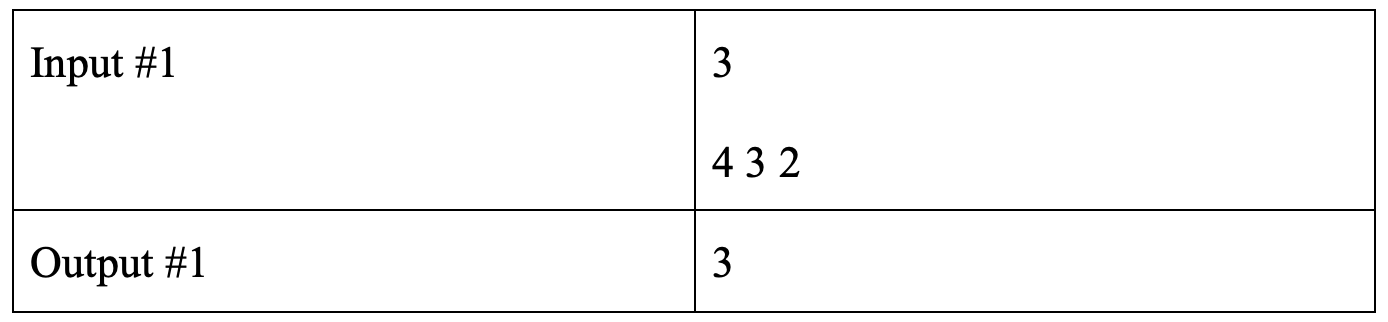
\includegraphics[width=0.80\textwidth]{q1_iodata.png}
    \end{figure}

\vspace{5pt}

\paragraph{实验环境}
\begin{itemize}
    \item 程序设计语言:C++
    \item 编程环境:
    \begin{itemize}
        \item 编辑器:Visual Studio Code (1.67.0)
        \item 编译器:g++ (GCC) 11.2.0
        \item 操作系统:ArchLinux 5.17.5-zen1-1-zen (64-bit)
    \end{itemize}
\end{itemize}

\vspace{5pt}

\paragraph{解答} 时间复杂度:$O(n \log n)$

源码:
\inputminted[bgcolor=codebg,frame=lines,autogobble,linenos=true,breaklines]{cpp}{src/t1.cpp}

\vspace{5pt}

\paragraph{实验结果}
(可附上截图)

\newpage

\subsection*{题目2:中位数}
\paragraph{题目内容}
\subparagraph{题目描述}
\begin{itemize}
    \item $X[1,2,..n]$和$Y[1,2,...,n]$为2个数组,每个数组含有n个已排好序的数字$(1 \leq n \leq 100)$。请采用分治法(算法复杂度可达O(logn))找出X和Y的2n个数的中位数。
\end{itemize}

\subparagraph{输入格式}
    \begin{itemize}
        \item 第一行输入一个数n,表示数组X或Y中元素个数。
        \item 第二行含有n个数字,以空格隔开,表示数组X中元素。
        \item 第三行含有n个数字,以空格隔开,表示数组Y中元素。
    \end{itemize}

\subparagraph{输出格式}
    \begin{itemize}
        \item 一个数字,表示数据X和Y的中位数。
    \end{itemize}
    
\subparagraph{输入输出样例}
    \begin{figure}[h]
        \centering
        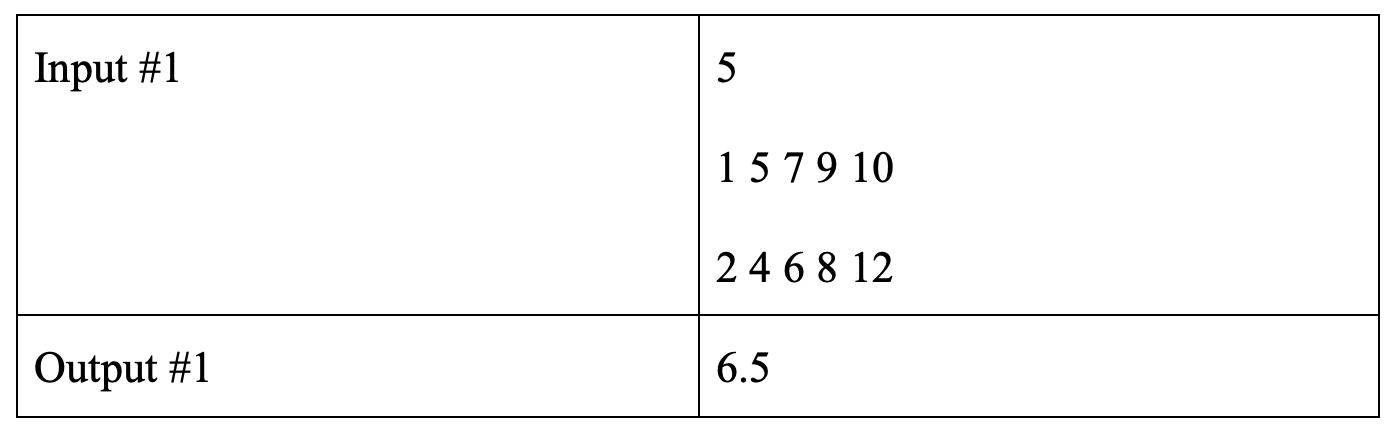
\includegraphics[width=0.80\textwidth]{q2_iodata.png}
    \end{figure}


\vspace{5pt}

\paragraph{实验环境}
\begin{itemize}
    \item 程序设计语言:C++
    \item 编程环境:
    \begin{itemize}
        \item 编辑器:Visual Studio Code (1.67.0)
        \item 编译器:g++ (GCC) 11.2.0
        \item 操作系统:ArchLinux 5.17.5-zen1-1-zen (64-bit)
    \end{itemize}
\end{itemize}

\vspace{5pt}

\paragraph{解答} 本题未成功解出

源码:
\inputminted[bgcolor=codebg,frame=lines,autogobble,linenos=true,breaklines]{cpp}{src/t2.cpp}

\vspace{5pt}

\paragraph{实验结果}
未成功解出

\newpage

\subsection*{题目3:分治法-出头数}
\paragraph{题目内容}
\subparagraph{题目描述}

\begin{itemize}
    \item 给定n个整数$(1 \leq n \leq 100)$,采用分治法,找到其中的出头元素。出头元素是指在数组中出现次数大于$\frac{n}{2}$(向下取整)的元素。(给定的数组总是存在出头元素)。
\end{itemize}

\subparagraph{输入格式}
    \begin{itemize}
        \item 第一行输入一个整数n,表示待输入元素个数。
        \item 第二行输入n个整数,以空格隔开。
    \end{itemize}

\subparagraph{输出格式}
    \begin{itemize}
        \item 出头元素。
    \end{itemize}
    

\subparagraph{输入输出样例}
    \begin{figure}[h]
        \centering
        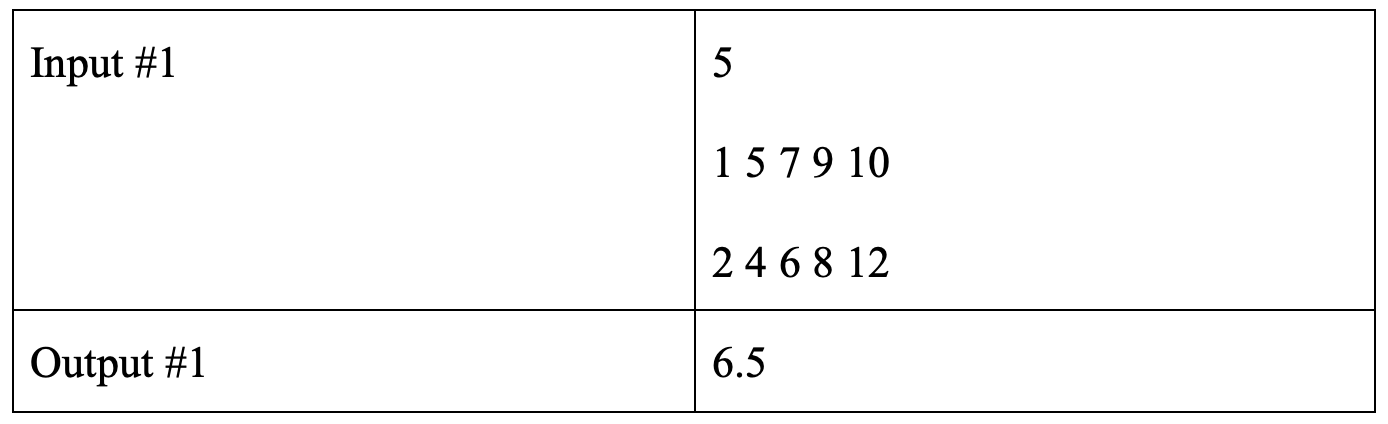
\includegraphics[width=0.80\textwidth]{q3_iodata.png}
    \end{figure}

\vspace{5pt}

\paragraph{实验环境}
\begin{itemize}
    \item 程序设计语言:C++
    \item 编程环境:
    \begin{itemize}
        \item 编辑器:Visual Studio Code (1.67.0)
        \item 编译器:g++ (GCC) 11.2.0
        \item 操作系统:ArchLinux 5.17.5-zen1-1-zen (64-bit)
    \end{itemize}
\end{itemize}

\vspace{5pt}

\paragraph{解答} 时间复杂度:$O(n)$

源码:
\inputminted[bgcolor=codebg,frame=lines,autogobble,linenos=true,breaklines]{cpp}{src/t3.cpp}

\vspace{5pt}

\paragraph{实验结果}
(可附上截图)

\newpage

\section*{三、心得体会}
    可根据“实验思考”部分作答,也可以根据个人具体体会作答。自己算法的创新点可在此处进行介绍,酌情加分。

\end{document} 
